\section*{Dijkstra's Algorithm~(continued)}


We rewrite the formula in Corollary~1~(last Lecture) into an equivalent form by separating the minimization into two levels:
$$distance(s, v_{k+1}^*) = \textstyle \min_{v\in V\setminus R_k} \min_{u\in R_k, (u, v)\in E} (distance(s, u) + l(u,v)).$$
Now we define the inner level of minimization with a new term $dist_k(v)$:
$$dist_k(v) := \textstyle \min_{u\in R_k, (u, v)\in E} (distance(s, u) + l(u,v)).$$
Then we have 
$$distance(s, v_{k+1}^*) = \textstyle \min_{v\in V\setminus R_k} dist_k(v).$$
Intuitively, $dist_k(v)$ gives the length of the shortest path from $s$ to $v$ by only using vertices in $R_k$.

\begin{figure}[h]
\centering{

\tikzset{every picture/.style={line width=0.75pt}} %set default line width to 0.75pt        

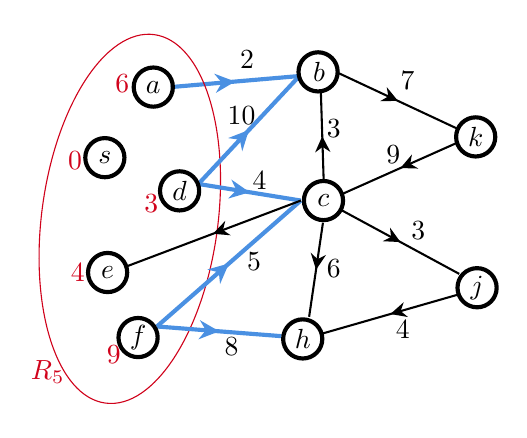
\begin{tikzpicture}[x=0.5pt,y=0.5pt,yscale=-1,xscale=1]
%uncomment if require: \path (0,296); %set diagram left start at 0, and has height of 296

%Straight Lines [id:da3320252336737717] 
\draw [color={rgb, 255:red, 74; green, 144; blue, 226 }  ,draw opacity=1 ][line width=1.5]    (119,48) -- (212,40) ;
\draw [shift={(165.5,44)}, rotate = 535.0799999999999] [fill={rgb, 255:red, 74; green, 144; blue, 226 }  ,fill opacity=1 ][line width=0.08]  [draw opacity=0] (14.56,-6.99) -- (0,0) -- (14.56,6.99) -- (9.67,0) -- cycle    ;
%Shape: Ellipse [id:dp2857420369455096] 
\draw  [color={rgb, 255:red, 208; green, 2; blue, 27 }  ,draw opacity=1 ] (26.24,134.88) .. controls (35.95,61.34) and (72.1,5.46) .. (106.98,10.07) .. controls (141.87,14.67) and (162.28,78.02) .. (152.57,151.56) .. controls (142.86,225.1) and (106.71,280.98) .. (71.83,276.37) .. controls (36.94,271.77) and (16.53,208.42) .. (26.24,134.88) -- cycle ;
%Straight Lines [id:da02943457575339692] 
\draw [color={rgb, 255:red, 74; green, 144; blue, 226 }  ,draw opacity=1 ][line width=1.5]    (139,118) -- (212,40) ;
\draw [shift={(175.5,79)}, rotate = 493.1] [fill={rgb, 255:red, 74; green, 144; blue, 226 }  ,fill opacity=1 ][line width=0.08]  [draw opacity=0] (14.56,-6.99) -- (0,0) -- (14.56,6.99) -- (9.67,0) -- cycle    ;
%Straight Lines [id:da7032022658079198] 
\draw [color={rgb, 255:red, 74; green, 144; blue, 226 }  ,draw opacity=1 ][line width=1.5]    (139,118) -- (213,130) ;
\draw [shift={(176,124)}, rotate = 189.21] [fill={rgb, 255:red, 74; green, 144; blue, 226 }  ,fill opacity=1 ][line width=0.08]  [draw opacity=0] (14.56,-6.99) -- (0,0) -- (14.56,6.99) -- (9.67,0) -- cycle    ;
%Straight Lines [id:da9416797747261806] 
\draw [color={rgb, 255:red, 74; green, 144; blue, 226 }  ,draw opacity=1 ][line width=1.5]    (109,221) -- (213,130) ;
\draw [shift={(161,175.5)}, rotate = 498.81] [fill={rgb, 255:red, 74; green, 144; blue, 226 }  ,fill opacity=1 ][line width=0.08]  [draw opacity=0] (14.56,-6.99) -- (0,0) -- (14.56,6.99) -- (9.67,0) -- cycle    ;
%Straight Lines [id:da6197316893700862] 
\draw [color={rgb, 255:red, 74; green, 144; blue, 226 }  ,draw opacity=1 ][line width=1.5]    (109,221) -- (199,228) ;
\draw [shift={(154,224.5)}, rotate = 184.45] [fill={rgb, 255:red, 74; green, 144; blue, 226 }  ,fill opacity=1 ][line width=0.08]  [draw opacity=0] (14.56,-6.99) -- (0,0) -- (14.56,6.99) -- (9.67,0) -- cycle    ;
%Straight Lines [id:da7705917014251779] 
\draw [color={rgb, 255:red, 0; green, 0; blue, 0 }  ,draw opacity=1 ][line width=0.75]    (86,178) -- (213,130) ;
\draw [shift={(149.5,154)}, rotate = 339.3] [fill={rgb, 255:red, 0; green, 0; blue, 0 }  ,fill opacity=1 ][line width=0.08]  [draw opacity=0] (11.61,-5.58) -- (0,0) -- (11.61,5.58) -- (7.71,0) -- cycle    ;
%Straight Lines [id:da7178806242260687] 
\draw [color={rgb, 255:red, 0; green, 0; blue, 0 }  ,draw opacity=1 ][line width=0.75]    (326,78) -- (240.5,38) ;
\draw [shift={(283.25,58)}, rotate = 205.07] [fill={rgb, 255:red, 0; green, 0; blue, 0 }  ,fill opacity=1 ][line width=0.08]  [draw opacity=0] (11.61,-5.58) -- (0,0) -- (11.61,5.58) -- (7.71,0) -- cycle    ;
%Straight Lines [id:da2873203830948724] 
\draw [color={rgb, 255:red, 0; green, 0; blue, 0 }  ,draw opacity=1 ][line width=0.75]    (326.5,88) -- (243.5,125) ;
\draw [shift={(285,106.5)}, rotate = 335.97] [fill={rgb, 255:red, 0; green, 0; blue, 0 }  ,fill opacity=1 ][line width=0.08]  [draw opacity=0] (11.61,-5.58) -- (0,0) -- (11.61,5.58) -- (7.71,0) -- cycle    ;
%Straight Lines [id:da9325647569597147] 
\draw [color={rgb, 255:red, 0; green, 0; blue, 0 }  ,draw opacity=1 ][line width=0.75]    (327.5,183) -- (242.5,137) ;
\draw [shift={(285,160)}, rotate = 208.42] [fill={rgb, 255:red, 0; green, 0; blue, 0 }  ,fill opacity=1 ][line width=0.08]  [draw opacity=0] (11.61,-5.58) -- (0,0) -- (11.61,5.58) -- (7.71,0) -- cycle    ;
%Straight Lines [id:da8240281406202591] 
\draw [color={rgb, 255:red, 0; green, 0; blue, 0 }  ,draw opacity=1 ][line width=0.75]    (219,214) -- (229,146) ;
\draw [shift={(224,180)}, rotate = 278.37] [fill={rgb, 255:red, 0; green, 0; blue, 0 }  ,fill opacity=1 ][line width=0.08]  [draw opacity=0] (11.61,-5.58) -- (0,0) -- (11.61,5.58) -- (7.71,0) -- cycle    ;
%Straight Lines [id:da6386544223700206] 
\draw [color={rgb, 255:red, 0; green, 0; blue, 0 }  ,draw opacity=1 ][line width=0.75]    (229,226) -- (326.5,198) ;
\draw [shift={(277.75,212)}, rotate = 343.98] [fill={rgb, 255:red, 0; green, 0; blue, 0 }  ,fill opacity=1 ][line width=0.08]  [draw opacity=0] (11.61,-5.58) -- (0,0) -- (11.61,5.58) -- (7.71,0) -- cycle    ;
%Straight Lines [id:da7268529078901531] 
\draw [color={rgb, 255:red, 0; green, 0; blue, 0 }  ,draw opacity=1 ][line width=0.75]    (229.5,115) -- (227.5,52) ;
\draw [shift={(228.5,83.5)}, rotate = 448.18] [fill={rgb, 255:red, 0; green, 0; blue, 0 }  ,fill opacity=1 ][line width=0.08]  [draw opacity=0] (11.61,-5.58) -- (0,0) -- (11.61,5.58) -- (7.71,0) -- cycle    ;

% Text Node
\draw (16,244) node [anchor=north west][inner sep=0.75pt]   [align=left] {$\displaystyle \textcolor[rgb]{0.82,0.01,0.11}{R}\textcolor[rgb]{0.82,0.01,0.11}{_{5}}$};
% Text Node
\draw (43,93) node [anchor=north west][inner sep=0.75pt]   [align=left] {$\displaystyle \textcolor[rgb]{0.82,0.01,0.11}{0}$};
% Text Node
\draw (167.24,20.06) node [anchor=north west][inner sep=0.75pt]   [align=left] {$\displaystyle 2$};
% Text Node
\draw  [line width=1.5]   (71.38, 99) circle [x radius= 14.15, y radius= 14.15]   ;
\draw (71.38,99) node   [align=left] {$\displaystyle s$};
% Text Node
\draw (77,37) node [anchor=north west][inner sep=0.75pt]   [align=left] {$\displaystyle \textcolor[rgb]{0.82,0.01,0.11}{6}$};
% Text Node
\draw  [line width=1.5]   (106.38, 48) circle [x radius= 14.15, y radius= 14.15]   ;
\draw (106.38,48) node   [align=left] {$\displaystyle a$};
% Text Node
\draw (98,124) node [anchor=north west][inner sep=0.75pt]   [align=left] {$\displaystyle \textcolor[rgb]{0.82,0.01,0.11}{3}$};
% Text Node
\draw  [line width=1.5]   (125.38, 123) circle [x radius= 14.15, y radius= 14.15]   ;
\draw (125.38,123) node   [align=left] {$\displaystyle d$};
% Text Node
\draw (45,174) node [anchor=north west][inner sep=0.75pt]   [align=left] {$\displaystyle \textcolor[rgb]{0.82,0.01,0.11}{4}$};
% Text Node
\draw  [line width=1.5]   (73.38, 182) circle [x radius= 14.15, y radius= 14.15]   ;
\draw (73.38,182) node   [align=left] {$\displaystyle e$};
% Text Node
\draw  [line width=1.5]   (225.48, 37) circle [x radius= 14.15, y radius= 14.15]   ;
\draw (219.98,37) node [anchor=west] [inner sep=0.75pt]   [align=left] {$\displaystyle b$};
% Text Node
\draw  [line width=1.5]   (229.38, 130) circle [x radius= 14.15, y radius= 14.15]   ;
\draw (229.38,130) node   [align=left] {$\displaystyle c$};
% Text Node
\draw  [line width=1.5]   (339.38, 84) circle [x radius= 14.15, y radius= 14.15]   ;
\draw (339.38,84) node   [align=left] {$\displaystyle k$};
% Text Node
\draw  [line width=1.5]   (214.38, 230) circle [x radius= 14.15, y radius= 14.15]   ;
\draw (214.38,230) node   [align=left] {$\displaystyle h$};
% Text Node
\draw (71,233) node [anchor=north west][inner sep=0.75pt]   [align=left] {$\displaystyle \textcolor[rgb]{0.82,0.01,0.11}{9}$};
% Text Node
\draw  [line width=1.5]   (95.38, 229) circle [x radius= 14.15, y radius= 14.15]   ;
\draw (95.38,229) node   [align=left] {$\displaystyle f$};
% Text Node
\draw  [line width=1.5]   (340.38, 193) circle [x radius= 14.15, y radius= 14.15]   ;
\draw (340.38,193) node   [align=left] {$\displaystyle j$};
% Text Node
\draw (158.24,60.06) node [anchor=north west][inner sep=0.75pt]   [align=left] {$\displaystyle 10$};
% Text Node
\draw (176.24,107.06) node [anchor=north west][inner sep=0.75pt]   [align=left] {$\displaystyle 4$};
% Text Node
\draw (172.24,166.06) node [anchor=north west][inner sep=0.75pt]   [align=left] {$\displaystyle 5$};
% Text Node
\draw (156,227.5) node [anchor=north west][inner sep=0.75pt]   [align=left] {$\displaystyle 8$};
% Text Node
\draw (283.24,35.06) node [anchor=north west][inner sep=0.75pt]   [align=left] {$\displaystyle 7$};
% Text Node
\draw (291,143) node [anchor=north west][inner sep=0.75pt]   [align=left] {$\displaystyle 3$};
% Text Node
\draw (279.75,215) node [anchor=north west][inner sep=0.75pt]   [align=left] {$\displaystyle 4$};
% Text Node
\draw (273,88.47) node [anchor=north west][inner sep=0.75pt]   [align=left] {$\displaystyle 9$};
% Text Node
\draw (230,70) node [anchor=north west][inner sep=0.75pt]   [align=left] {$\displaystyle 3$};
% Text Node
\draw (230,171) node [anchor=north west][inner sep=0.75pt]   [align=left] {$\displaystyle 6$};


\end{tikzpicture}

}
\caption{Try above formulas in Figure~\ref{fig:extension}.
Answer: $dist_5(b) = \min\{8, 13\} = 8$, $dist_5(c) = \min\{7, 14\} = 7$, $dist_5(h) = 17$, $dist_5(k) = \infty$, $dist_5(j) = \infty$;
hence $v_6^* = c$ and $distance(s,v_6^*) = dist_5(c) = 7$.}
\label{fig:extension}
\end{figure}

With $dist_k$ available, the next closest vertex, i.e., $v_{k+1}^*$ can be easily calculated
by picking the one with smallest $dist_k$ value.
More importantly, we can design a more efficient procedure
to calculate $dist_{k+1}$ in the next iteration by largely reusing $dist_k$.
To see that, recall its definition, for any $v\in V\setminus R_{k+1}$, we have 
$$dist_{k+1}(v) = \textstyle \min_{u\in R_{k+1}, (u, v)\in E} (distance(s, u) + l(u,v)).$$
Note that $R_{k+1} = R_k \cup \{v_{k+1}^*\}$. Hence
\begin{displaymath}
dist_{k+1}(v) = \left\{
\begin{array}{llllll}
\min\{ dist_k(v), distance(s, v_{k+1}^*) + l(v_{k+1}^*, v) \} & \textrm{ if } & (v_{k+1}^*, v) \in E \\
dist_k(v) & \textrm{ if } & (v_{k+1}^*, v) \not\in E
\end{array}
\right.
\end{displaymath}
In other words, when calculating $dist_{k+1}$, we only need to examine the out-edges of $v_{k+1}^*$
and update only if the use of $v_{k+1}^*$ leads to a shorter path. The pseudo-code of
calculating $dist_{k+1}$ from $dist_k$ is given below.
Before calling this updating procedure, $dist_{k+1}$ is first copied from $dist_k$.

\begin{minipage}{0.8\textwidth}
	\aaA {6}{procedure update-dist~($dist_k, v_{k+1}^*$)}\xxx
	\aaB {4}{for $(v_{k+1}^*, v) \in E$}\xxx
	\aaC {2}{if~($dist_k(v) > distance(s, v_{k+1}^*) + l(v_{k+1}^*, v)$)}\xxx
	\aad {$dist_{k+1}(v) = distance(s, v_{k+1}^*) + l(v_{k+1}^*, v)$;}\xxx
	\aac {end if;}\xxx
	\aab {end for;}\xxx
	\aaa {end procedure;}\xxx
\end{minipage}

Try above procedure with the example below.

\begin{figure}[h!]
\centering{

\tikzset{every picture/.style={line width=0.75pt}} %set default line width to 0.75pt        

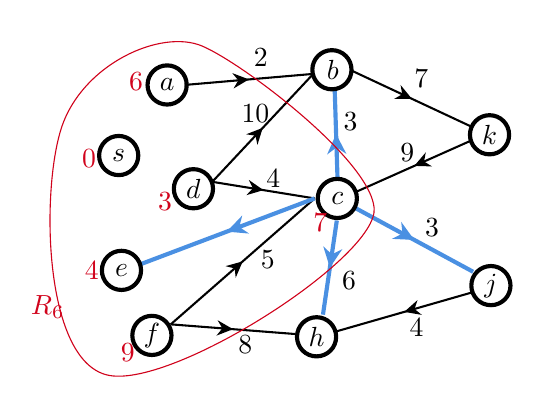
\begin{tikzpicture}[x=0.5pt,y=0.5pt,yscale=-1,xscale=1]
%uncomment if require: \path (0,284); %set diagram left start at 0, and has height of 284

%Straight Lines [id:da3320252336737717] 
\draw [color={rgb, 255:red, 0; green, 0; blue, 0 }  ,draw opacity=1 ][line width=0.75]    (242,47) -- (335,39) ;
\draw [shift={(288.5,43)}, rotate = 535.0799999999999] [fill={rgb, 255:red, 0; green, 0; blue, 0 }  ,fill opacity=1 ][line width=0.08]  [draw opacity=0] (11.61,-5.58) -- (0,0) -- (11.61,5.58) -- (7.71,0) -- cycle    ;
%Straight Lines [id:da02943457575339692] 
\draw [color={rgb, 255:red, 0; green, 0; blue, 0 }  ,draw opacity=1 ][line width=0.75]    (262,117) -- (335,39) ;
\draw [shift={(298.5,78)}, rotate = 493.1] [fill={rgb, 255:red, 0; green, 0; blue, 0 }  ,fill opacity=1 ][line width=0.08]  [draw opacity=0] (11.61,-5.58) -- (0,0) -- (11.61,5.58) -- (7.71,0) -- cycle    ;
%Straight Lines [id:da7032022658079198] 
\draw [color={rgb, 255:red, 0; green, 0; blue, 0 }  ,draw opacity=1 ][line width=0.75]    (262,117) -- (336,129) ;
\draw [shift={(299,123)}, rotate = 189.21] [fill={rgb, 255:red, 0; green, 0; blue, 0 }  ,fill opacity=1 ][line width=0.08]  [draw opacity=0] (11.61,-5.58) -- (0,0) -- (11.61,5.58) -- (7.71,0) -- cycle    ;
%Straight Lines [id:da9416797747261806] 
\draw [color={rgb, 255:red, 0; green, 0; blue, 0 }  ,draw opacity=1 ][line width=0.75]    (232,220) -- (336,129) ;
\draw [shift={(284,174.5)}, rotate = 498.81] [fill={rgb, 255:red, 0; green, 0; blue, 0 }  ,fill opacity=1 ][line width=0.08]  [draw opacity=0] (11.61,-5.58) -- (0,0) -- (11.61,5.58) -- (7.71,0) -- cycle    ;
%Straight Lines [id:da6197316893700862] 
\draw [color={rgb, 255:red, 0; green, 0; blue, 0 }  ,draw opacity=1 ][line width=0.75]    (232,220) -- (322,227) ;
\draw [shift={(277,223.5)}, rotate = 184.45] [fill={rgb, 255:red, 0; green, 0; blue, 0 }  ,fill opacity=1 ][line width=0.08]  [draw opacity=0] (11.61,-5.58) -- (0,0) -- (11.61,5.58) -- (7.71,0) -- cycle    ;
%Straight Lines [id:da7705917014251779] 
\draw [color={rgb, 255:red, 74; green, 144; blue, 226 }  ,draw opacity=1 ][line width=1.5]    (209,177) -- (336,129) ;
\draw [shift={(272.5,153)}, rotate = 339.3] [fill={rgb, 255:red, 74; green, 144; blue, 226 }  ,fill opacity=1 ][line width=0.08]  [draw opacity=0] (14.56,-6.99) -- (0,0) -- (14.56,6.99) -- (9.67,0) -- cycle    ;
%Straight Lines [id:da7178806242260687] 
\draw [color={rgb, 255:red, 0; green, 0; blue, 0 }  ,draw opacity=1 ][line width=0.75]    (449,77) -- (363.5,37) ;
\draw [shift={(406.25,57)}, rotate = 205.07] [fill={rgb, 255:red, 0; green, 0; blue, 0 }  ,fill opacity=1 ][line width=0.08]  [draw opacity=0] (11.61,-5.58) -- (0,0) -- (11.61,5.58) -- (7.71,0) -- cycle    ;
%Straight Lines [id:da2873203830948724] 
\draw [color={rgb, 255:red, 0; green, 0; blue, 0 }  ,draw opacity=1 ][line width=0.75]    (449.5,87) -- (366.5,124) ;
\draw [shift={(408,105.5)}, rotate = 335.97] [fill={rgb, 255:red, 0; green, 0; blue, 0 }  ,fill opacity=1 ][line width=0.08]  [draw opacity=0] (11.61,-5.58) -- (0,0) -- (11.61,5.58) -- (7.71,0) -- cycle    ;
%Straight Lines [id:da9325647569597147] 
\draw [color={rgb, 255:red, 74; green, 144; blue, 226 }  ,draw opacity=1 ][line width=1.5]    (450.5,182) -- (365.5,136) ;
\draw [shift={(408,159)}, rotate = 208.42] [fill={rgb, 255:red, 74; green, 144; blue, 226 }  ,fill opacity=1 ][line width=0.08]  [draw opacity=0] (14.56,-6.99) -- (0,0) -- (14.56,6.99) -- (9.67,0) -- cycle    ;
%Straight Lines [id:da8240281406202591] 
\draw [color={rgb, 255:red, 74; green, 144; blue, 226 }  ,draw opacity=1 ][line width=1.5]    (342,213) -- (352,145) ;
\draw [shift={(347,179)}, rotate = 278.37] [fill={rgb, 255:red, 74; green, 144; blue, 226 }  ,fill opacity=1 ][line width=0.08]  [draw opacity=0] (14.56,-6.99) -- (0,0) -- (14.56,6.99) -- (9.67,0) -- cycle    ;
%Straight Lines [id:da6386544223700206] 
\draw [color={rgb, 255:red, 0; green, 0; blue, 0 }  ,draw opacity=1 ][line width=0.75]    (352,225) -- (449.5,197) ;
\draw [shift={(400.75,211)}, rotate = 343.98] [fill={rgb, 255:red, 0; green, 0; blue, 0 }  ,fill opacity=1 ][line width=0.08]  [draw opacity=0] (11.61,-5.58) -- (0,0) -- (11.61,5.58) -- (7.71,0) -- cycle    ;
%Straight Lines [id:da7268529078901531] 
\draw [color={rgb, 255:red, 74; green, 144; blue, 226 }  ,draw opacity=1 ][line width=1.5]    (352.5,114) -- (350.5,51) ;
\draw [shift={(351.5,82.5)}, rotate = 448.18] [fill={rgb, 255:red, 74; green, 144; blue, 226 }  ,fill opacity=1 ][line width=0.08]  [draw opacity=0] (14.56,-6.99) -- (0,0) -- (14.56,6.99) -- (9.67,0) -- cycle    ;
%Shape: Polygon Curved [id:ds3197703892135201] 
\draw  [color={rgb, 255:red, 208; green, 2; blue, 27 }  ,draw opacity=1 ] (153,78) .. controls (168,32) and (225,6) .. (255,19) .. controls (285,32) and (376,101) .. (379,136) .. controls (382,171) and (236,265) .. (188,257) .. controls (140,249) and (138,124) .. (153,78) -- cycle ;

% Text Node
\draw (129,197) node [anchor=north west][inner sep=0.75pt]   [align=left] {$\displaystyle \textcolor[rgb]{0.82,0.01,0.11}{R}\textcolor[rgb]{0.82,0.01,0.11}{_{6}}$};
% Text Node
\draw (166,92) node [anchor=north west][inner sep=0.75pt]   [align=left] {$\displaystyle \textcolor[rgb]{0.82,0.01,0.11}{0}$};
% Text Node
\draw (290.24,19.06) node [anchor=north west][inner sep=0.75pt]   [align=left] {$\displaystyle 2$};
% Text Node
\draw  [line width=1.5]   (194.38, 98) circle [x radius= 14.15, y radius= 14.15]   ;
\draw (194.38,98) node   [align=left] {$\displaystyle s$};
% Text Node
\draw (200,36) node [anchor=north west][inner sep=0.75pt]   [align=left] {$\displaystyle \textcolor[rgb]{0.82,0.01,0.11}{6}$};
% Text Node
\draw  [line width=1.5]   (229.38, 47) circle [x radius= 14.15, y radius= 14.15]   ;
\draw (229.38,47) node   [align=left] {$\displaystyle a$};
% Text Node
\draw (221,123) node [anchor=north west][inner sep=0.75pt]   [align=left] {$\displaystyle \textcolor[rgb]{0.82,0.01,0.11}{3}$};
% Text Node
\draw  [line width=1.5]   (248.38, 122) circle [x radius= 14.15, y radius= 14.15]   ;
\draw (248.38,122) node   [align=left] {$\displaystyle d$};
% Text Node
\draw (168,173) node [anchor=north west][inner sep=0.75pt]   [align=left] {\textcolor[rgb]{0.82,0.01,0.11}{$\displaystyle 4$}};
% Text Node
\draw  [line width=1.5]   (196.38, 181) circle [x radius= 14.15, y radius= 14.15]   ;
\draw (196.38,181) node   [align=left] {$\displaystyle e$};
% Text Node
\draw  [line width=1.5]   (348.48, 36) circle [x radius= 14.15, y radius= 14.15]   ;
\draw (342.98,36) node [anchor=west] [inner sep=0.75pt]   [align=left] {$\displaystyle b$};
% Text Node
\draw  [line width=1.5]   (352.38, 129) circle [x radius= 14.15, y radius= 14.15]   ;
\draw (352.38,129) node   [align=left] {$\displaystyle c$};
% Text Node
\draw  [line width=1.5]   (462.38, 83) circle [x radius= 14.15, y radius= 14.15]   ;
\draw (462.38,83) node   [align=left] {$\displaystyle k$};
% Text Node
\draw  [line width=1.5]   (337.38, 229) circle [x radius= 14.15, y radius= 14.15]   ;
\draw (337.38,229) node   [align=left] {$\displaystyle h$};
% Text Node
\draw (194,232) node [anchor=north west][inner sep=0.75pt]   [align=left] {$\displaystyle \textcolor[rgb]{0.82,0.01,0.11}{9}$};
% Text Node
\draw  [line width=1.5]   (218.38, 228) circle [x radius= 14.15, y radius= 14.15]   ;
\draw (218.38,228) node   [align=left] {$\displaystyle f$};
% Text Node
\draw  [line width=1.5]   (463.38, 192) circle [x radius= 14.15, y radius= 14.15]   ;
\draw (463.38,192) node   [align=left] {$\displaystyle j$};
% Text Node
\draw (281.24,59.06) node [anchor=north west][inner sep=0.75pt]   [align=left] {$\displaystyle 10$};
% Text Node
\draw (299.24,106.06) node [anchor=north west][inner sep=0.75pt]   [align=left] {$\displaystyle 4$};
% Text Node
\draw (295.24,165.06) node [anchor=north west][inner sep=0.75pt]   [align=left] {$\displaystyle 5$};
% Text Node
\draw (279,226.5) node [anchor=north west][inner sep=0.75pt]   [align=left] {$\displaystyle 8$};
% Text Node
\draw (406.24,34.06) node [anchor=north west][inner sep=0.75pt]   [align=left] {$\displaystyle 7$};
% Text Node
\draw (414,142) node [anchor=north west][inner sep=0.75pt]   [align=left] {$\displaystyle 3$};
% Text Node
\draw (402.75,214) node [anchor=north west][inner sep=0.75pt]   [align=left] {$\displaystyle 4$};
% Text Node
\draw (396,87.47) node [anchor=north west][inner sep=0.75pt]   [align=left] {$\displaystyle 9$};
% Text Node
\draw (355,65) node [anchor=north west][inner sep=0.75pt]   [align=left] {$\displaystyle 3$};
% Text Node
\draw (354,180) node [anchor=north west][inner sep=0.75pt]   [align=left] {$\displaystyle 6$};
% Text Node
\draw (333.24,138.06) node [anchor=north west][inner sep=0.75pt]   [align=left] {$\displaystyle \textcolor[rgb]{0.82,0.01,0.11}{7}$};


\end{tikzpicture}

}
\caption{Following Figure~\ref{fig:extension}, we have that $v_6^* = c$.
We now want to calculate $dist_6$ using $dist_5$. We consider the out-edges of $c$, marked as thick blue edges.
Eventually, $dist_6(b) = 8$, $dist_6(h) = 13$, $dist_6(k) = \infty$, and $dist_6(j) = 10$.  }
\label{fig:update}
\end{figure}

The above procedure enables fast calculation of $dist_k$.
The last piece of Dijkstra's algorithm comes with the use of \emph{priority queue}
to quickly pick the next closest vertex, i.e., to calculate $v_{k+1}^* = \arg\min_{v\in V\setminus R_k} dist_k(v)$.
To this end, the priority queue $PQ$ always stores $V\setminus R_k$,
and for each vertex $v$ that is stored in $PQ$, its priority is $dist_k(v)$.
In this way, every time we call find-min~($PQ$), it gives us $\min_{v\in V\setminus R_k} dist_k(v)$.
In the complete Dijkstra's algorithm, we don't need to implicitly maintain $R_k$,
as $PQ$ is always complement to $R_k$.
In order to maintain this invariant, we delete $v_{k+1}^*$ from $PQ$, by calling delete-min, at the time of adding $v_{k+1}^*$ to $R_{k+1}$.
In order to guarantee that the priority of $v$ is always $dist_k(v)$,
we call decrease-key every time we update $dist_k$ of a vertex.

\begin{minipage}{0.8\textwidth}
	\aaA {16}{Algorithm Dijkstra~($G = (V, E)$, $l(e)$ for any $e\in E$, $s \in V$)}\xxx
	\aab {$dist[v] = \infty$, for any $v\in V$;}\xxx
	\aab {init an empty priority queue $PQ$;}\xxx
	\aab {for any $v\in V$: insert~($PQ$, $v$), where the priority of $v$ is $\infty$;}\xxx
	\aab {$dist[s] = 0$;}\xxx
	\aab {decrease-key~($PQ, s, 0$);}\xxx
	\aaB {9}{while~(empty~($PQ$) = false)}\xxx
	\aac {$u$ = find-min~($PQ$);}\xxx
	\aac {delete-min~($PQ$);}\xxx
	\aaC {5}{for each edge~$(u, v)\in E$}\xxx
	\aaD {3}{if~($dist[v] > dist[u] + l(u,v)$)}\xxx
	\aae {$dist[v] = dist[u] + l(u,v)$;}\xxx
	\aae {decrease-key~($PQ$, $v$, $dist[v]$);}\xxx
	\aad {end if;}\xxx
	\aac {end for;}\xxx
	\aab {end while;}\xxx
	\aaa {end algorithm;}\xxx
\end{minipage}

The pseudo-code for complete Dijkstra's algorithm is given above.
We use array $dist$ of size $n$ to store $dist_k$.
Where are the distances for those vertices in $R_k$~(i.e., those are not in $PQ$) stored?
They are in array $dist$ as well.
This is because, at the time $v_{k+1}^*$ is identified and added to $R_{k+1}$~(i.e., removed from $PQ$),
$dist_k$ value for this vertex is exactly its distance.
In fact, at any time of the algorithm, $dist[v] = distance(s,v)$ for any vertex $v$ that is not in $PQ$.
Finally, the algorithm don't explicitly maintain an index $k$: this index implicitly increases in every iteration of the while loop.


Here are some facts about Dijkstra's algorithm.
First, $dist[v]$ is always an upper bound of the distance.
\begin{fact} \label{fact1}
At any time of the algorithm, $dist[v] \ge distance(s,v)$.
\end{fact}

This is because, by definition, $dist_k(v)$ is the length of 
shortest path from $s$ to $v$ using only vertices in $R_k$.
In other words, $dist_k(v)$ represents the length of the optimal
path of a subset~(of all possible paths from $s$ to $v$).

Second, once $v$ is removed from $PQ$, $dist[v]$ won't change and remain as $distance(s,v)$.
\begin{fact}
At any time of the algorithm, if $v$ is not in $PQ$, then $dist[v] = distance(s,v)$.
\end{fact}
This is because, at the time $v$ is deleted from $PQ$, $dist[v] = distance(s,v)$.
Following Fact~\ref{fact1}, it will remain this minimized value.
Notice though, in Dijkstra's algorithm, a vertex $v$ not in $PQ$ might be ``touched''
by an edge $(v^*_{k+1}, v)$, where $v^*_{k+1}$ is the newly determined closest vertex,
   but the actual update will not happen.
See an example in Figure~2 of Lecture 17, edge~$(c, e)$.
%Such ``attempts'' to reduce $dist[v]$ will always fail.

The running time of Dijkstra's algorithmd depends on the specific implementation of priority queue used.
Consider using binary heap. The break-down of running time is given below.
Note that each vertex will be picked from the $PQ$ at most once and each edge will be examined at most once~(for directed graph) or at most twice~(for undirected graph).
The total running time is $\Theta((|V|+|E|)\log |V|)$.
\vspace*{-\topsep}
\begin{enumerate}
\item initialization: $\Theta(|V|)$;
\item insert~($PQ$): $|V| \times \Theta(\log |V|)$;
\item empty~($PQ$): $|V| \times \Theta(1)$;
\item find-min~($PQ$): $|V| \times \Theta(1)$;
\item delete-min~($PQ$): $|V| \times \Theta(\log |V|)$;
\item updating-dist: $|E| \times \Theta(1)$;
\item decrease-key~($PQ$): $|E| \times \Theta(\log |V|)$;
\end{enumerate}

\section*{Properties of Shortest Path Problem}

To prepare to solve the shortest path problem with negative edge length, we first see some properties.

A negative cycle $C$ in a graph is a cycle with negative length, i.e., $l(C) := \sum_{e\in C} l(e) < 0$.
In the presence of negative cycle, if we don't limit the number of edges
in a path, then the length of a path could goes to negative infinity.
In other words, the shortest path may not exist.
Therefore, in a graph with negative edge length, we want to
detect if there exists negative cycle.
We will show an algorithm~(the Bellman-Ford algorithm) can be used to detect negative cycles.

A path $p$ in a graph is \emph{simple} if $p$ does not have repeating vertices.
If a graph $G$ does not contain negative cycle, then 
for any pair of vertices $u$ and $v$, if $u$ can reach $v$,
then there always exists a {simple} shortest path from $u$ to $v$,
as otherwise we can skip the cycle in it to get a better or same-length path.
If all cycles in graph $G$ are positive then every shortest path is simple.

\begin{property}
If $G$ does not contain negative cycles, for every $u,v\in V$, there exists a shortes path
from $u$ to $v$ with at most $(|V| - 1)$ edges.
\end{property}

Shortest path admits the following \emph{optimal substructure} property.
Intuitively, this property states that, the shortest path from $u$ to $v$
contains the shortest path from $u$ to any internal vertex on this path~(formally described below).
Essentially, this is why shortest path problem can be solved efficiently.

\begin{property}
Let $p = (v_1, v_2) \to (v_2, v_3) \to \cdots \to (v_{k-1}, v_k)$
be the shortest path from $v_1$ to $v_k$.
Then for any $1\le i \le k$,
$p_i := (v_1, v_2) \to (v_2, v_3) \to \cdots \to (v_{i-1}, v_i)$, i.e., the portion of $p$ from $v_1$ to $v_i$,
is the shortest path from $v_1$ to $v_i$.
\end{property}

\emph{Proof.} Suppose that 
$p_i = (v_1, v_2) \to (v_2, v_3) \to \cdots \to (v_{i-1}, v_i)$
is not the shortest path from $v_1$ to $v_i$. Assume that
$q$ is the shorest path from $v_1$ to $v_i$.
Then we can construct a path from $v_1$ to $v_k$ shorter than $p$,
by concatenating $q$ and $(v_i, v_{i+1}) \to \cdots \to (v_{k-1}, v_k)$.
This contradicts to the fact that $p$ is the shortest path from $v_1$ to $v_k$.\qed

Note that the above property holds even for graphs with negative edge length~(as
in the proof we don't assume anything about edge length).
This property also immediately implies the following fact.

\begin{property}
If we know that there exists one shortest path from $s$ to $v$ such that $(w,v)$ is the last edge
on this shortest path, then we have that $distanct(s,v) = distance(s,w) + l(w,v)$.
\end{property}
